%Plantilla para articulo en ingles con comandos personalizados David Davalos.
\documentclass[letterpaper,12pt]{article} % {{{
%Para compilar con MikTex cambiar los siguientes dos paquetes por \usepackage[latin1]{inputenc}
\usepackage{ucs}
\usepackage[utf8x]{inputenc} 
%\usepackage[spanish]{babel}
%\spanishdecimal{.}
\usepackage{color}                    
\usepackage{graphicx} 
\usepackage{url}
\usepackage{bm} %Greek bf
\usepackage{anysize}
\usepackage{amsmath}
\usepackage{amssymb}
\usepackage{multicol}  
\newcommand{\one}{\mathbbm{1}}
\usepackage{texdraw}  
\usepackage{float}
\usepackage{fancyhdr}
\usepackage{amsfonts}
\usepackage{cancel}
\usepackage[usenames,dvipsnames]{pstricks}
%\usepackage{epsfig}
%\usepackage{pst-grad} % For gradients
\usepackage{pst-plot}
\usepackage{hyperref}
%%%%% De la tesis %%%%%%%%%%
%\usepackage[sc]{mathpazo} % Esta es la fuente chida!
%\usepackage[addendum]{stix}
\usepackage{lettrine}
\usepackage{amsthm}
\usepackage{xcolor}
%\usepackage{pdfpages}
\usepackage{url}
\usepackage{tikz}
%%%%%%%%%%%%%%%%%%%%%%%%%%%%%
\newcommand{\<}{\langle}
\newcommand{\mcU}{\mathcal{U}}
\newcommand{\mcA}{\mathcal{A}}
\newcommand{\mcO}{\mathcal{O}}
\newcommand{\mcI}{\mathcal{I}}
\newcommand{\mcH}{\mathcal{H}}
\newcommand{\mcM}{\mathcal{M}}
\newcommand{\mcN}{\mathcal{N}}
\newcommand{\mcQ}{\mathcal{Q}}
\newcommand{\mcE}{\mathcal{E}}
\newcommand{\mcC}{\mathcal{C}}
\newcommand{\mcJ}{\mathcal{J}}
\usepackage{bbm}
\newcommand{\mcK}{\mathcal{K}}
\newcommand{\mcB}{\mathcal{B}}
\newcommand{\mcL}{\mathcal{L}}
\newcommand{\mcF}{\mathcal{F}}
\newcommand{\mcT}{\mathcal{T}}
\newcommand{\mcS}{\mathcal{S}}
\newcommand{\mcD}{\mathcal{D}}
\newcommand{\diag}{\text{diag}}
\newcommand{\ie}{i.e.}
\newcommand{\eg}{\textit{e.g.}}
\newcommand{\ipr}{\mathrm{ipr}}
\newcommand{\rmH}{\mathrm{H}}
\newcommand{\rmq}{\mathrm{q}}
\newcommand{\cut}{\mathrm{cut}}
\newcommand{\rmd}{\mathrm{d}}
\newcommand{\rmi}{\mathrm{i}}
%\newcommand{\red}{\color{red}}
\newcommand{\rmf}{f}
%\newcommand{\eg}{\textit{e.g.} }
%\newcommand{\Eg}{\textit{E.g.} }
\newcommand{\eref}[1]{eq.~(\ref{#1})} 
\newcommand{\sref}[1]{sec.~\ref{#1}}
\newcommand{\fref}[1]{fig.~\ref{#1}}
\newcommand{\tref}[1]{table~\ref{#1}}
\newcommand{\Eref}[1]{Eq.~(\ref{#1})} 
\newcommand{\Sref}[1]{Sec.~\ref{#1}}
\newcommand{\Fref}[1]{Fig.~\ref{#1}}  
\newcommand{\Tref}[1]{Table~\ref{#1}}
\newcommand{\Or}{\mathord{\mathrm{O}} }
\newcommand{\tr}{\mathop{\mathrm{tr}}\nolimits}
\newcommand{\comm}[1]{{\color{red} #1 }}
\newcommand{\qv}{QV}
\newcommand{\old}{\infty}
\newcommand{\Mmed}{\mcM^{\<\cdot\>}}
\newcommand{\MBLP}{\mcM^{\text{BLP}} }
\newcommand{\MRHP}{\mcM^{\text{RHP}} }
%\newcommand{\blue}{\color{blue}}
\newcommand{\note}[1]{{\color{orange}\textbf{#1}}\\}

\newcommand{\ket}[1]{{\vert #1 \rangle}}
\newcommand{\bra}[1]{{\langle #1 \vert}}
\newcommand{\proj}[2]{{\vert #1 \rangle \langle #2 \vert}}
\newcommand{\cp}{\color{red}   }
\graphicspath{{images/}}
\newcommand{\fig}[1]{fig.\ref{#1}}
\newcommand{\eqn}[1]{eqn.\eqref{#1}}
\newcommand{\tab}[1]{table \ref{#1}}
\newcommand{\id}{\t}
\newtheorem{theorem}{Theorem}
\newtheorem{proposition}{Proposition}
\newtheorem{definition}{Definition}
%%Si no esta usando el iop package
%%Si no esta usando el iop package
%%Si no esta usando el iop package
%\input{definiciones}
%Comandos mios generales
\newcommand{\fig}[1]{fig.\ref{#1}}
\newcommand{\eqn}[1]{eqn.\eqref{#1}}
\newcommand{\tab}[1]{table \ref{#1}}
\newcommand{\medline}{\begin{center}\line(1,0){470}\end{center}}
\newcommand{\suspensivos}{{\color{blue} (.....)}}
\newcommand{\anotacion}[1]{{\color{red} (.. #1 ...)}}
\newcommand{\ie}{\textit{i. e.}}
%Quantum Mechanics Commands
\newcommand{\ket}[1]{{\vert #1 \rangle}}
\newcommand{\bra}[1]{{\langle #1 \vert}}
\newcommand{\proj}[2]{{\vert #1 \rangle \langle #2 \vert}}
\newcommand{\NoM}{{\cal N}}
%Lugares
\newcommand{\unam}{Universidad Nacional Aut\'onoma de M\'exico, M\'exico, D.F., M\'exico}
\newcommand{\icf}{Instituto de Ciencias F\'{\i}sicas, \unam}
\newcommand{\ifunam}{Instituto de F\'{\i}sica, \unam}
\newcommand{\ifunamint}{Instituto de F\'{\i}´ısica, Universidad Nacional Aut\'onoma de M\'exico, M\'exico D.F. 01000, M\'exico}
\newcommand{\fcen}{Departamento de F\'isica ``J. J. Giambiagi'', FCEN, Universidad de Buenos Aires, 1428 Buenos Aires, Argentina}
%%%%%%%%%%% Comandos de Carlos %%%%%%%%%%%%%%%%%%%%%%%%
% enges
%%%%%%%%%%%%%
%%%%%%%%%%%
\newif\ifenglish
\newif\ifespanol
\newif\ifshort
\newif\iflong
\shorttrue
\englishtrue
\newcommand{\enges}[2]{\ifenglish #1 \fi \ifespanol #2 \fi}
%%%%%%
%%%%%

%Comandos mios generales
\newcommand{\fig}[1]{fig.\ref{#1}}
\newcommand{\eqn}[1]{eqn.\eqref{#1}}
\newcommand{\tab}[1]{table \ref{#1}}
\newcommand{\medline}{\begin{center}\line(1,0){470}\end{center}}
\newcommand{\suspensivos}{{\color{blue} (.....)}}
\newcommand{\anotacion}[1]{{\color{red} (.. #1 ...)}}
\newcommand{\ie}{\textit{i. e.}}
%Quantum Mechanics Commands
\newcommand{\ket}[1]{{\vert #1 \rangle}}
\newcommand{\bra}[1]{{\langle #1 \vert}}
\newcommand{\proj}[2]{{\vert #1 \rangle \langle #2 \vert}}
\newcommand{\NoM}{{\cal N}}
%Lugares
\newcommand{\unam}{Universidad Nacional Aut\'onoma de M\'exico, M\'exico, D.F., M\'exico}
\newcommand{\icf}{Instituto de Ciencias F\'{\i}sicas, \unam}
\newcommand{\ifunam}{Instituto de F\'{\i}sica, \unam}
\newcommand{\ifunamint}{Instituto de F\'{\i}´ısica, Universidad Nacional Aut\'onoma de M\'exico, M\'exico D.F. 01000, M\'exico}
\newcommand{\fcen}{Departamento de F\'isica ``J. J. Giambiagi'', FCEN, Universidad de Buenos Aires, 1428 Buenos Aires, Argentina}
%%%%%%%%%%% Comandos de Carlos %%%%%%%%%%%%%%%%%%%%%%%%
% enges
%%%%%%%%%%%%%
%%%%%%%%%%%
\newif\ifenglish
\newif\ifespanol
\newif\ifshort
\newif\iflong
\shorttrue
\englishtrue
\newcommand{\enges}[2]{\ifenglish #1 \fi \ifespanol #2 \fi}
%%%%%%
%%%%%

%Comandos mios generales
\newcommand{\fig}[1]{fig.\ref{#1}}
\newcommand{\eqn}[1]{eqn.\eqref{#1}}
\newcommand{\tab}[1]{table \ref{#1}}
\newcommand{\medline}{\begin{center}\line(1,0){470}\end{center}}
\newcommand{\suspensivos}{{\color{blue} (.....)}}
\newcommand{\anotacion}[1]{{\color{red} (.. #1 ...)}}
\newcommand{\ie}{\textit{i. e.}}
%Quantum Mechanics Commands
\newcommand{\ket}[1]{{\vert #1 \rangle}}
\newcommand{\bra}[1]{{\langle #1 \vert}}
\newcommand{\proj}[2]{{\vert #1 \rangle \langle #2 \vert}}
\newcommand{\NoM}{{\cal N}}
%Lugares
\newcommand{\unam}{Universidad Nacional Aut\'onoma de M\'exico, M\'exico, D.F., M\'exico}
\newcommand{\icf}{Instituto de Ciencias F\'{\i}sicas, \unam}
\newcommand{\ifunam}{Instituto de F\'{\i}sica, \unam}
\newcommand{\ifunamint}{Instituto de F\'{\i}´ısica, Universidad Nacional Aut\'onoma de M\'exico, M\'exico D.F. 01000, M\'exico}
\newcommand{\fcen}{Departamento de F\'isica ``J. J. Giambiagi'', FCEN, Universidad de Buenos Aires, 1428 Buenos Aires, Argentina}
%%%%%%%%%%% Comandos de Carlos %%%%%%%%%%%%%%%%%%%%%%%%
% enges
%%%%%%%%%%%%%
%%%%%%%%%%%
\newif\ifenglish
\newif\ifespanol
\newif\ifshort
\newif\iflong
\shorttrue
\englishtrue
\newcommand{\enges}[2]{\ifenglish #1 \fi \ifespanol #2 \fi}
%%%%%%
%%%%%

%comandos locales
\marginsize{1.5 cm}{1.5 cm}{-0.5 cm}{1 cm}
\author{David Davalos}                                 
\date{\today}                                
\title{Notes on erasing maps}     
\begin{document} 
\maketitle
\tableofcontents
\newpage
\section{Analysis of entanglement distribution of JAs channels}
Here we analyze the fidelity distribution of one element on each class, since they are connected trivially through local unitaries, it is enough to consider  one element per class.
\begin{figure}[H]
\centering
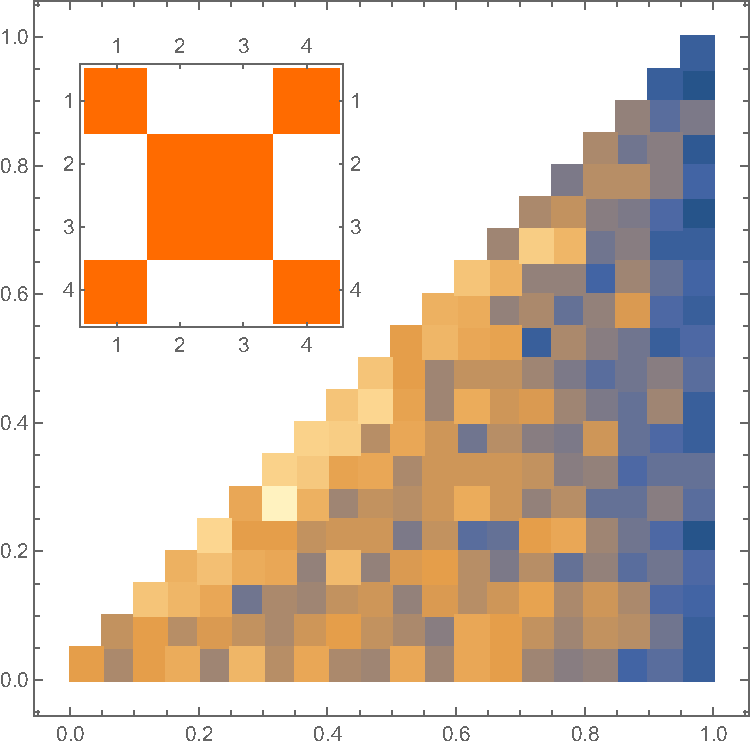
\includegraphics[scale=0.5]{distro_1.pdf}
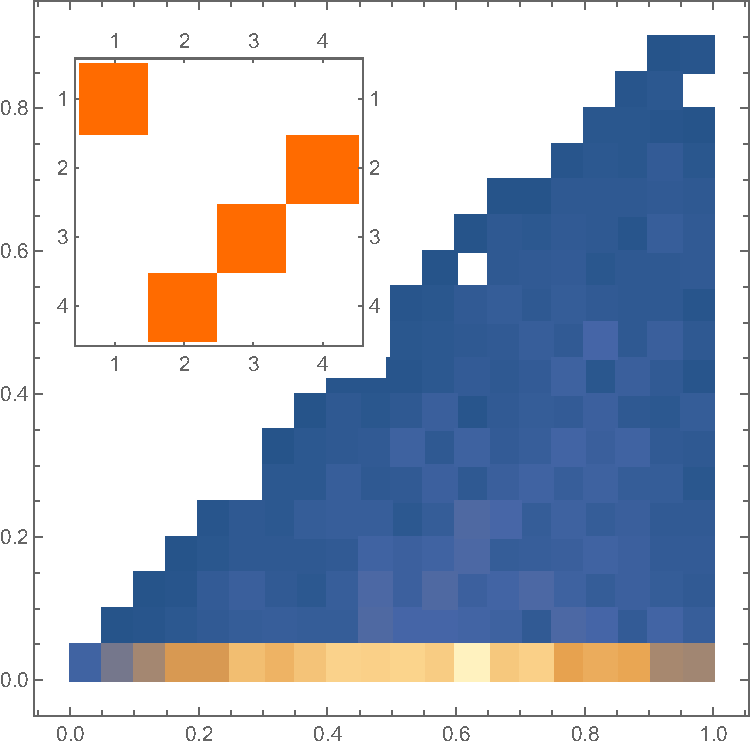
\includegraphics[scale=0.5]{distro_2.pdf}
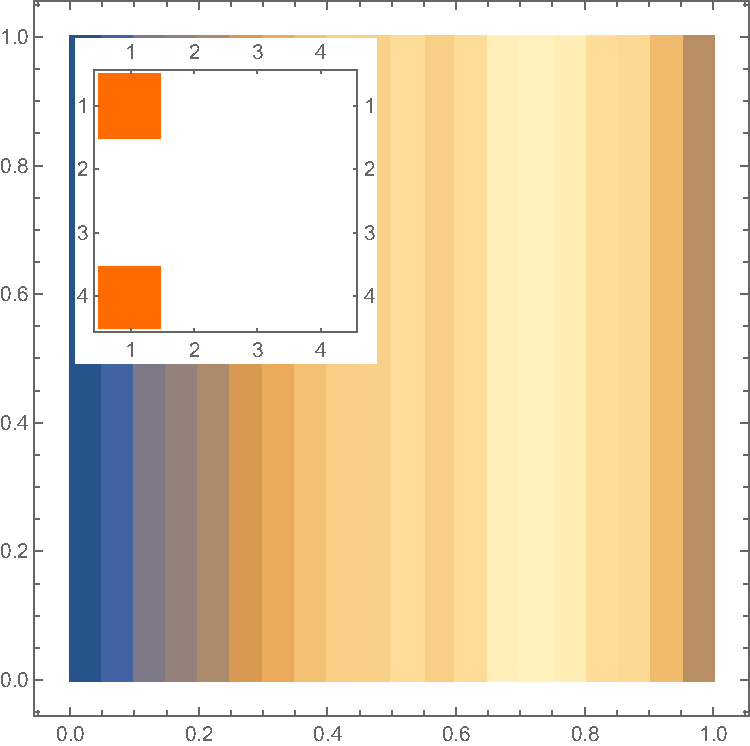
\includegraphics[scale=0.5]{distro_triv.pdf}
\caption{eje x: concurrencia inicial, eje y: concurrencia final, tomando estados aleatorios.}
\end{figure}
\section{Erasing correlations plus local? noise}
Let's define the mappings parameterized by $\mu$:
\begin{equation}
\mcE:\sum_{i,j} r_{ij} (\sigma_i \otimes \sigma_j) \mapsto \sum_{i>0} \mu r_{i0} (\sigma_i\otimes \one) +\sum_{i>0} \mu r_{0i} (\one \otimes \sigma_i)+r_{00} \one\otimes \one
\end{equation}
We found that such mappings are CPTP if and only if
\begin{equation}
-\frac{1}{6}\leq \mu\leq \frac{1}{2}.
\end{equation}
Defining similar maps for $3$ and $4$ particles respectively, we have:
\begin{align}
-\frac{1}{36}\leq &\mu\leq \frac{1}{4},\\
-\frac{1}{174}\leq &\mu \leq \frac{1}{10}\\
\end{align}
The last one doesn't follow the elegance of the growing dimension, this must be checked again. All this was computed analytically using mathematica.

\section{Exploring and writing the former maps}
Consider the map
\begin{equation}
\rho \mapsto (1-\mu) \tr_B \rho \otimes \sigma_1+\mu \sigma_2 \otimes \tr_A \rho,
\end{equation}
Taking $\sigma_1=\sigma_2=\one_{2 \times 2}/2$, we have that the map takes $\vec r$ to:
\begin{equation}
\left(
\begin{array}{cccc}
 r_{0,0} & \mu  r_{0,1} & \mu  r_{0,2} & \mu  r_{0,3} \\
 (1-\mu) r_{1,0} & 0 & 0 & 0 \\
 (1-\mu) r_{2,0} & 0 & 0 & 0 \\
 (1-\mu) r_{3,0} & 0 & 0 & 0 \\
\end{array}
\right)
\end{equation}
\bibliographystyle{alpha}
\bibliography{labibliografia} 
\end{document}

%Thrash
\section{Implementing approximations to erasing using partial traces}
The non-physical mapping (it violates the non-Broadcasting theorem) is defined as follows
\begin{align}
\rho &\mapsto \tr_B \rho \otimes \tr_A \rho\\
&= \tr_{2,3} \left( \rho \otimes \rho\right)\\
&= \tr_{2,3}\circ \mcC[\rho],
\end{align}
where
\begin{equation}
\mcC[\rho]=\rho \otimes \rho
\end{equation}
is a cloning map.  It violates the non-broadvasting theorem and naturally it is not CPTP. An approximate CPTP map can be found in principle using various strategies. We use here the one for finding the approximate universal NOT gate and the approximate transposition map, this is, by adding isotropic noise to the density matrix,
\begin{align}
\rho &\mapsto \mcC'[\rho]\nonumber \\
&= (1-\mu) \rho \otimes \rho + \mu \tr \rho \frac{\one}{4}.
\end{align}
This channel is CPTP if and only if
\begin{equation}
\frac{4 \sqrt{3}-4}{4 \sqrt{3}-3}\leq \mu \leq \frac{4 \sqrt{3}+4}{4 \sqrt{3}+3}.
\end{equation}
This was computed in mathematica imposing the positive-semidefinitvness of the Choi matrix.
Still constructing the rectangular map including the trace.
